\section{Bakti QIlan Mufid | 1174083}
\subsection{Soal 1}
Apa itu fungsi device manager di windows dan folder /dev di linux.
\begin{itemize}
	\item Device Manager: Device Manager dalam komputer windows, adalah perluasan dari Microsoft Management Console. Device Manager menampilkan seluruh hardware yang bisa di-inisialisasi (dikenali) oleh Windows. dan fungsi dari Device Manager ini ialah dalam mengelola (manage) semua hardware yang terpasang (dan terdeteksi)dalam suatu sistem Windows. Hardware seperti harddisk, kartu VGA, sound, keyboard, perangkat USB dll. akan sangat mudah untuk dikonfigurasi dari dalam Device Manager ini. Device Manager paling sering digunakan untuk pengelolaan driver suatu hardware. Misalnya instalasi driver, uninstal driver, update driver, rollback driver, dan bermacam problem yang berkaitan dengan driver suatu hardware.
	\item folder /dev berisi semua drive harddisk atau hardware seperti modem, CD/DVD/Blu-ray dsb. Hanya saja disini hanya merupakan link dan bukan isi, contohnya hdd partisi 1 ada di /dev/sda1 dan DVD-rom ada di /dev/sr0. untuk melihat isinya, harus dilakukan mounting (mount) terlebih dahulu.
\end{itemize}

\subsection{Soal 2}

Jelaskan langkah-langkah instalasi driver dari arduino UNO di Windows

Berikut ini adalah langkah-langkah instalasi driver dari arduino UNO di Windows
	\begin{itemize}
		\item Pertama pastikan Arduino IDE telah terinstall.
		\item Hubungkan port USB Arduino Uno ke port USB PC.
			\begin{figure}[ht]
				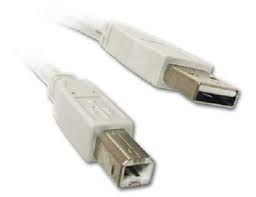
\includegraphics[width=10cm]{figures/5/1174083/Teori/kabel.jpg}
				\centering
				\caption{menghubungkan port.}
			\end{figure}
		\item Lalu pada bagian kanan didesktop PC anda, akan muncul popup “Installing device driver software” seperti pada gambar dibawah ini.
			\begin{figure}[ht]
				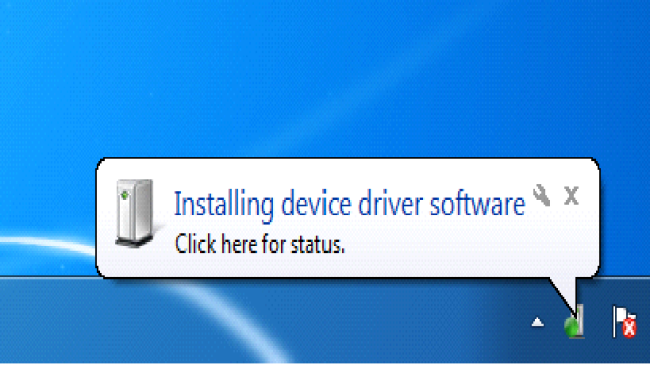
\includegraphics[width=10cm]{figures/5/1174083/Teori/2.png}
				\centering
				\caption{muncul pop up.}
			\end{figure}
		\item SIstem operasi Windows tidak menyediakan driver untuk Arduino Uno seperti yang terlihat pada gambar dibawah ini, lalu proses instalasinya harus dilakukan secara manual.
			\begin{figure}[ht]
				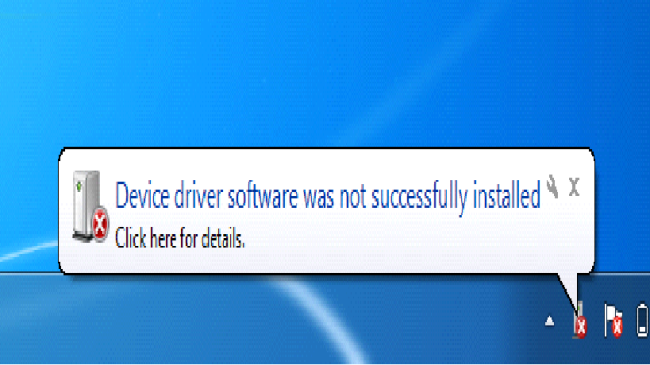
\includegraphics[width=10cm]{figures/5/1174083/Teori/3.png}
				\centering
				\caption{instalasi manual.}
			\end{figure}
		\item Buka Device Manager, caranya pada bagian Search Program and Files lalu ketikkan “device manager” (tanpa tanda petik), perhatikan gambar dibawah ini. Pada bagian Control Panel akan muncul Device Manager, klik untuk menjalankan.
			\begin{figure}[ht]
				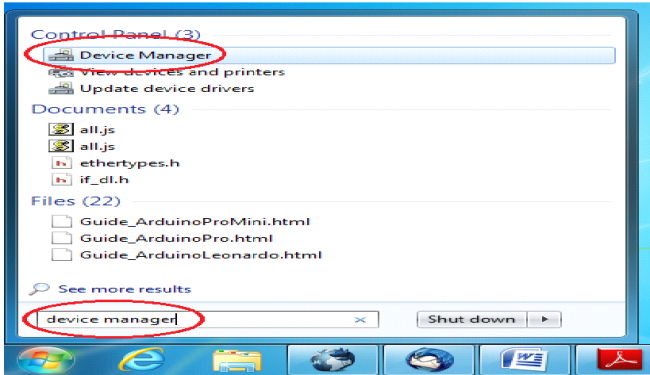
\includegraphics[width=10cm]{figures/5/1174083/Teori/4.png}
				\centering
				\caption{membuka device manager.}
			\end{figure}
		\item Cari Unknown device pada bagian Other device, biasanya terdapat tanda seru berwarna kuning, itu disebabkan karena penginstallan tidak berjalan dengan sempurna.
			\begin{figure}[ht]
				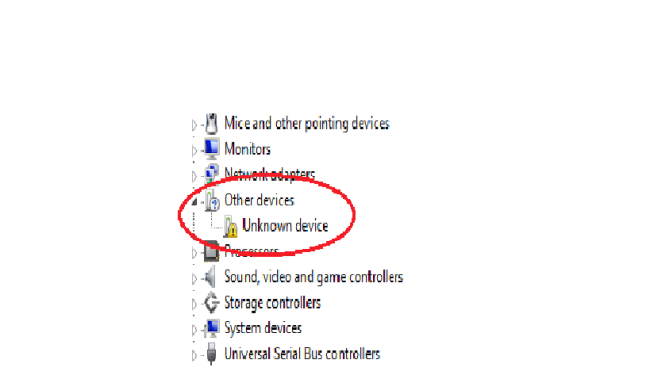
\includegraphics[width=10cm]{figures/5/1174083/Teori/5.png}
				\centering
				\caption{tanda seru.}
			\end{figure}
		\item Klik kanan pada “Unknown device” kemudian pilih Update Driver Software.		
			\begin{figure}[ht]
				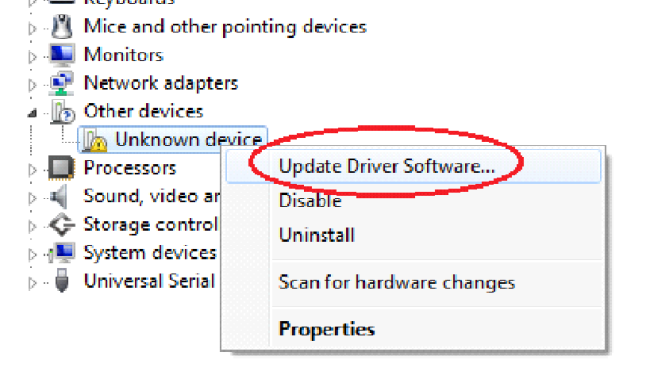
\includegraphics[width=10cm]{figures/5/1174083/Teori/6.png}
				\centering
				\caption{update Driver Software.}
			\end{figure}
		\item Pilih Browse my computer for driver software.
			\begin{figure}[ht]
				\includegraphics[width=10cm]{figures/5/1174083/Teori/7.png}
				\centering
				\caption{Browse my computer.}
			\end{figure}
		\item Arahkan lokasi folder ke folder \verb|..\arduino-1.0.5\drivers.| Pastikan check-box lalu centang include subfolders. Klik Next untuk melanjutkan instalasi driver.
			\begin{figure}[ht]
				\includegraphics[width=10cm]{figures/5/1174083/Teori/8.png}
				\centering
				\caption{mengarahkan lokasi ke folder.}
			\end{figure}
		\item Kemudian lanjutkan dengan mengklik Install pada tampilan Windows Security.
			\begin{figure}[ht]
				\includegraphics[width=10cm]{figures/5/1174083/Teori/9.png}
				\centering
				\caption{Klik Install.}
			\end{figure}
		\item Jika instalasi driver berhasil maka akan muncul Windows has successfully updated your driver software.
			\begin{figure}[ht]
				\includegraphics[width=10cm]{figures/5/1174083/Teori/10.png}
				\centering
				\caption{Successfully}
			\end{figure}
		\item Perhatikan dan ingat nama COM Arduino Uno, karena nama COM ini yang akan digunakan untuk meng-upload program nantinya.
			\begin{figure}[ht]
				\includegraphics[width=10cm]{figures/5/1174083/Teori/11.png}
				\centering
				\caption{Selesai.}
			\end{figure}
	\end{itemize}
	
\subsection{Soal 3}
Jelaskan bagaimana cara membaca baudrate dan port dari komputer yang sudah
terinstall driver

Untuk melihat atau membaca baudrate dan port kita hanya perlu menginstall Arduino IDE, setelah itu buka menu serial monitor yang berada di tab tools. Dari sana akan terlihat baik baudrate dan port yang sedang digunakan oleh arduino anda.

\subsection{Soal 4}
Jelaskan sejarah library pyserial

PySerial merupakan sebuah library yang digunakan untuk komunikasi ke port serial terutama untuk mikrokontroller. PySerial pertama kali diluncurkan pada tahun 2002 yang makin berkembang dalam setiap versinya hingga tahun 2017 lalu.

\subsection{Soal 5}
Jelaskan fungsi-fungsi apa saja yang dipakai dari library pyserial

Fungsi-fungsi yang dipakai dari library PySerial, yaitu:
\begin{enumerate}
	\item Serial - fungsi ini untuk membuka port serial.
	\item read(size) - fungsi ini untuk membaca jumlah byte dari port serial.
	\item write(data) - fungsi ini menulis data lewat port serial.
	\item readline() - fungsi ini membaca sebuah string dari port serial.
	\item close() - fungsi ini untuk menutup port serial.
\end{enumerate}

\subsection{Soal 6}
Jelaskan kenapa butuh perulangan dan tidak butuh perulangan dalam membaca serial

Karena dalam pembacaan serial dalam arduino yang memerlukan membaca data secara berulang-ulang harus dengan perulangan. dan tidak butuh perulangan ketika membaca data hanya dilakukan sekali saja.

\subsection{Soal 7}
Jelaskan bagaimana cara membuat fungsi yang mengunakan pyserial

tata cara untuk membuat pyserial seperti pada kode dibawah

\lstinputlisting[firstline=10, lastline=16]{src/5/1174083/Teori/1174083.py}


\subsection{Cek Plagiat}
\begin{figure}[H]
	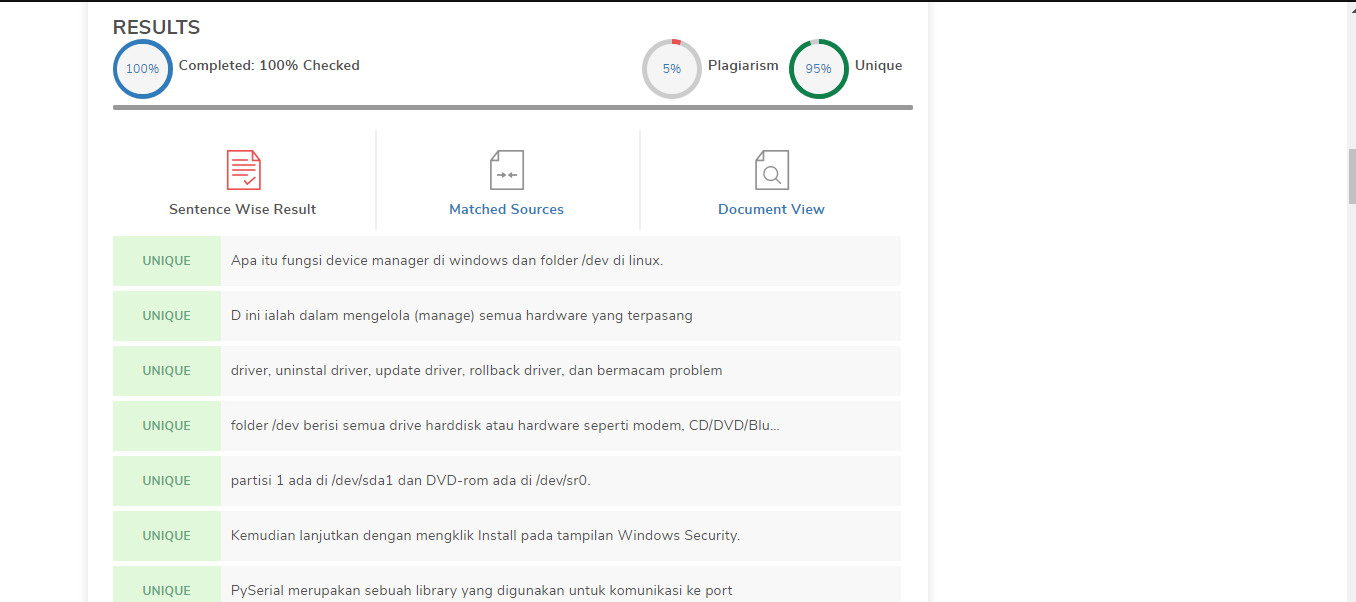
\includegraphics[width=10cm]{figures/5/1174083/Teori/plagiat1.png}
	\centering
	\caption{Hasil cek plagiarism.}
\end{figure}

\subsection{Kode Program}
\begin{figure}[ht]
	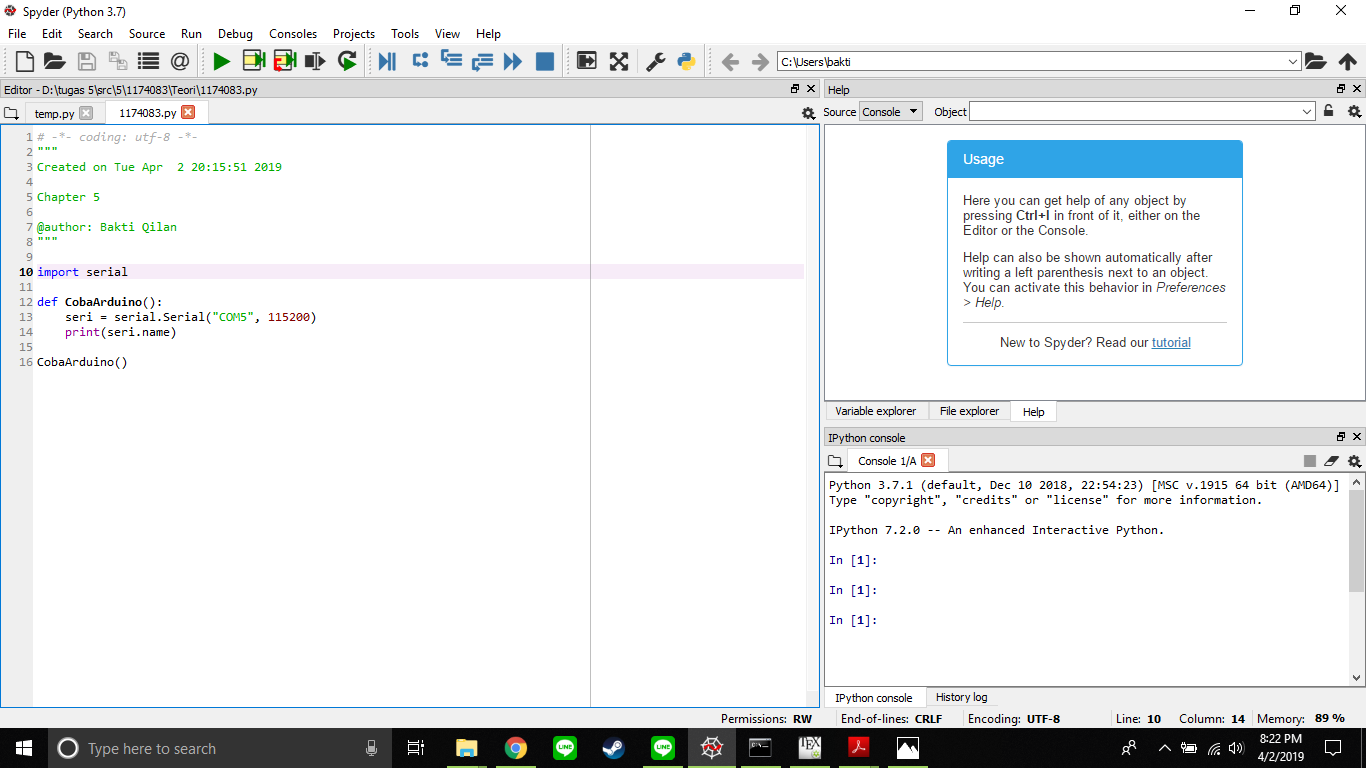
\includegraphics[width=10cm]{figures/5/1174083/Teori/kodefungsi.png}
	\centering
	\caption{Kode program fungsi.}
\end{figure}

%%%%%%%%%%%%%%%%%%%%%%%%%%%%%%%%%%%%%%%%%%%%%%%%%%%%%%%%%%%%%%%%%%%%%%%%%%%%%%%%%%%%%%%%%%%%%%%%%%%%%%%%%
\section{Mochamad Arifqi Ramadhan | 1174074}
\subsection{Soal 1}

\textbf{Fungsi Device manager di Windows  Folder /dev di Linux}
\begin{itemize}
\item Fungsi Device Manager di Windows
	Device Manager akan sangat membantu dalam mengelola (manage) semua hardware yang terpasang (dan terdeteksi) dalam suatu sistem Windows. Hardware seperti harddisk, kartu VGA, sound, keyboard, perangkat USB dll. akan sangat mudah untuk dikonfigurasi dari dalam Device Manager ini. ( mengetahui port arduinno)

\item Fungsi Folder /dev di Linux
/dev berfungsi mengetahui  direktori yang tersimpan konfigurasi device/hardware pada sistem. Contohnya folder /dev artinya file-file tersebut berada.
\end{itemize}
	
\subsection{Soal 2}	
\textbf{Intall Arduino}

Cara instalasi driver arduino :
		\begin{enumerate}
			\item Pertama download software arduino, extract bila file zip/rar
			\item hubungkan Port USB Arduino UNO ke Port USB PC
			\item lalu windows akan memunculkan pop up yang memberitahu bahwa ingin menginstall dirver, tapi nanti tidak akan menemukan drivernya
			\item buka Device Manager, setelah Device Manager terbuka, silahkan cari “Unknown Device” yang berada di Other Device.
			\item klik kanan pada unknown device tersebut lalu pilih update driver software
			\item pilih browse my computer for driver software lalu masukkan directory dimana anda menyimpan driver arduino yang telah anda download tadi
			\item setelah itu klik install dan tunggu hingga proses selesai
			\item arduino pun sudah terbaca di pc anda 
		\end{enumerate}


\subsection{Soal 3}

\textbf{Membaca baudrate dan port di komputer}
Untuk membaca baudrate dan port di komputer pertama hbungkan arduino dengan komputer
1. bisa dengan cara membuka Device manager
2. lalu pilih ports (COM  dan LPT)
3. pilih COM yang terhubung
4. Pilih port setting dan lihat di Bit per second untuk baudrate

Sedangkan untuk port
lakukan proses 1 dan 2 seperti diatas
Dan port dari arduino telah terbaca oleh PC
	
\subsection{Soal 4}

\textbf{Sejarah library PySerial}

	PySerial adalah library yang menyediakan dukungan untuk koneksi serial ("RS-232") melalui berbagai perangkat yang berbeda: port serial gaya lama, dongle Bluetooth, port infra merah, dan sebagainya. Ini juga mendukung port serial jarak jauh melalui RFC 2217 (sejak V2.5). dan PySerial pertama kali diluncurkan pada tahun 2002 yang makin berkembang dalam setiap versinya hingga tahun 2017 lalu.

\subsection{Soal 5}

\textbf{Fungsi-Fungsi di library PySerial}
\begin{itemize}
\item print(ser.name)         - meriksa port yang benar-benar digunakan
\item ser.write(b'hello')     	- menulis tipe data string
\item ser.readline()  	- untuk membaca string dari port serial
\item  ser.read()         	 - membaca satu port
\item ser.close()         	- menutup port
\end{itemize}

\subsection{Soal 6}

\textbf{Perulangan dan Tidak Perulangan}
	Perulangan digunakan untuk melakukan scanning/pengambilan data secara terus menerus(continue) artinya pengeksekusiannya terus berjalan auto selama ada scanning/pengambilan data. Sedangkan Tidak Pengulangan digunakan untuk menscanning/pengambilan data secara real time atau pengambilan datanya hanya sekali saja.


\subsection{Soal 7}

\textbf{Membuat fungsi dengan PySerial}


 Import Serial

Ser = serial.Serial (port, baudrate) membuka serial port
Ketengan : Ser adalah objek Serial, serial adalah kelas, Serial adalah method

contoh fungsi : data = Ser.readline() artinya membaca data


\subsection{Bukti Screenshoot}

\begin{figure}[H]
	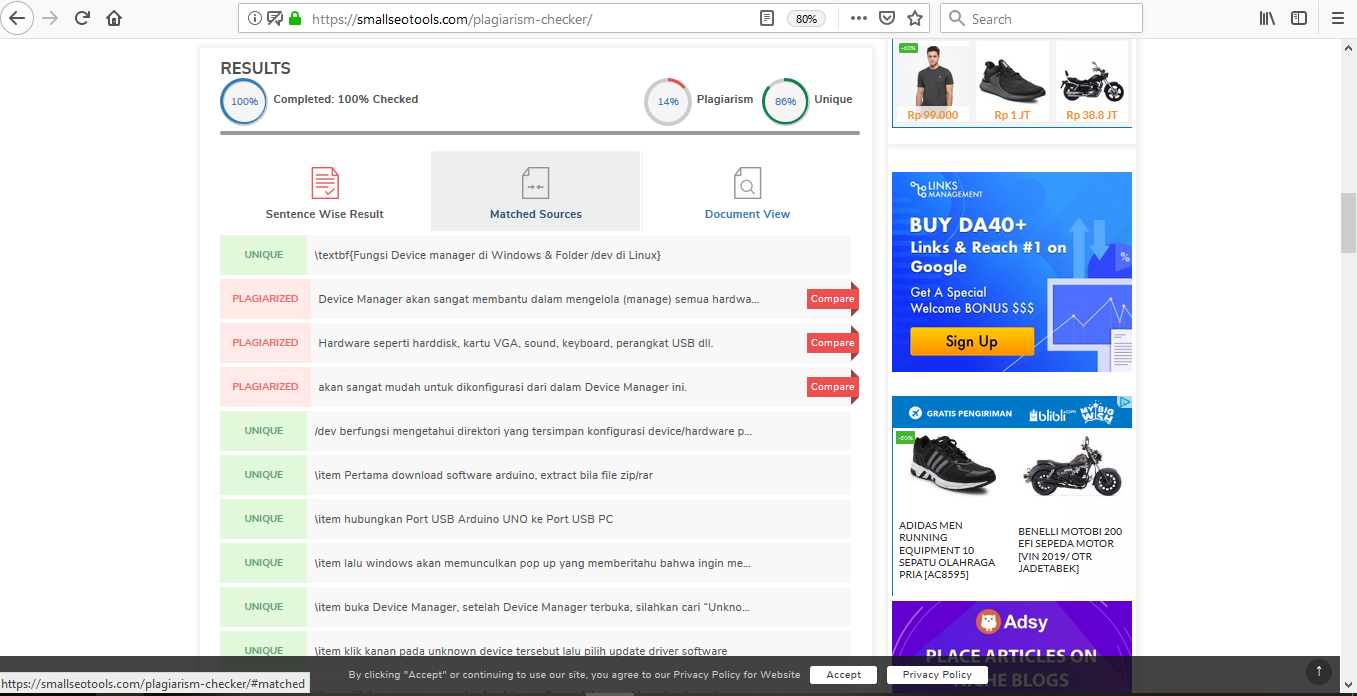
\includegraphics[width=10cm]{figures/5/1174074/Teori/plagiarisme2.png}
	\centering	
	\caption{Cek Plagiat}
\end{figure}
%%%%%%%%%%%%%%%%%%%%%%%%%%%%%%%%%%%%%%%%%%%%%%%%%%%%%%%%%%%%%%%%%%%%%%%%%%%%%%%%%%%%%%%%%%%%%%%%%%%%%%%%%%%%%%%%%%%%


\section{Dini Permata Putri}
\begin{enumerate}

\item Apa itu fungsi device manager di windows dan folder /dev di linux.\\
jawab : \\
Device Manager dalam komputer Windows, adalah perluasan dari Microsoft Management Console. Device Manager menampilkan seluruh hardware yang bisa di-inisialisasi (dikenali) oleh Windows. Tampilannya sudah ter-organisir (dikelompokkan) sedemikian rupa sehingga akan memudahkan pengelolaan setiap hardware yang ada.\\

Fungsi Device Manager Windows\\
Device Manager akan sangat membantu dalam mengelola (manage) semua hardware yang terpasang (dan terdeteksi) dalam suatu sistem Windows. Hardware seperti harddisk, kartu VGA, sound, keyboard, perangkat USB dll. akan sangat mudah untuk dikonfigurasi dari dalam Device Manager ini.\\
folder /dev di linux
Directory ini berisi file device, baik device blok maupun device karakter. di dalamnya minimal harus ada file biner MAKEDEV untuk membuat device ini secara manual.\\

\item Jelaskan langkah-langkah instalasi driver dari arduino\\
jawab :\\
- setalah anda berhasil mengunduh file installer (sekitar 80 Mb), double click-lah file tersebut untuk segera memulai proses instalasi\\
- setelah file installer dijalankan, akan muncul jendela 'Licanse Agreement'. Klik aja tombol 'I Agree'\\
- berikutnya anda akan diminta memasukan folder instalasi Arduino. Biarkan default di C:/Program Files/Arduino. atau kalau mau diganti juga bisa\\
- setelah itu akan muncul jendela 'Setup Installation Options'. Sebaiknya dicentang semua opsinya\\
- selanjutnya proses instalasi dimulai\\
- ditengah proses instalasi, jika komputer anda belum terinstal driver USB, maka akan muncul jendela 'Security Warning' sbb. click tombol instal.\\
- tunggu sampai proses instalasi 'Complated'\\
- pada tahap ini software IDE Arduino sudah terinstal. coba cek di Start Menu Windows anda atau di desktop seharusnya ada ikon Arduino. jika sudah menemukannya, jalankan aplikasi tersebut. dan muncul splash screen\\
- beberapa detik kemudian, jendela IDE Arduino akan muncul\\

\item Jelaskan bagaimana cara membaca baudrate dan port dari komputer yag sudah terinstall driver\\
jawab : \\
untuk membaca baudrate menggunakan Arduino IDE, sedangkan membaca port menggunakan device manager\\

\item Jelaskan sejarah library pyserial\\
jawab :\\
Pyserial adalah library/modul Python siap-pakai dan gratis yang dibuat untuk memudahkan kita dalam membuat program komunikasi data serial RS232 dalam bahasa Python.\\

Jika modul USB-2REL dapat kita kontrol dengan mudah menggunakan Python dan PyUSB (lihat pembahasannya di sini dan di sini), maka modul SER-2REL juga dapat kita kontrol dengan mudah menggunakan Python dengan bantuan modul PySerial.\\

\item jelaskan fungsi-fungsi apa saja yang dipakai dari library pyserial\\
jawab :\\
- SER2REL = serial.Serial(“COM1”, 2400)\\

Jika binding berhasil maka port serial COM1 akan di-open dan siap digunakan. Untuk mengetes apakah COM1 sudah open dan siap digunakan, kita gunakan fungsi isOpen sebagai berikut:\\

- SER2REL.isOpen()\\

Fungsi ini menghasilkan nilai True jika COM1 sudah open dan nilai False jika sebaliknya. Pada eksperimen kita, SER2REL.isOpen() menghasilkan nilai True yang berarti kita sudah dapat mengirim dan menerima data ke dan dari port serial COM1.\\

\item Jelaskan kenapa butuh perulangan dalam tidak butuh perulangan dalam membaca serial\\
jawab :\\
Perulangan atau dalam istilah lain disebut dengan loop. Perulangan digunakan ketika kamu harus menyelesaikan sebuah task dengan jumlah yang besar dengan menggunakan pola yang sama. Syaratnya tentu saja, kamu harus mengetahui bagaimana pola atau alur dari task tersebut. \\

Di dalam Python, ada dua jenis perulangan yang lazim digunakan, yaitu:\\

- For\\
Adalah suatu bentuk perulangan yang mengerjakan ”bagian pernyatan yang sama” secara berulang kali berdasarkan syarat/kondisi yang ditentukan. Cara kerja ini digunakan untuk menyelesaikan task dengan cara yang sama dan dengan hasil yang berbeda.\\

- While\\
Digunakan  untuk melakukan task perulangan selama kondisi nya bernilai benar. Logika pengecakan adalah sama dengan statement IF untuk menentukan benar atau salah. Berikut ini adalah struktur dari while\\

\item Jelaskan bagaimana cara meembuat fungsi yang menggunakan pyserial\\
jawab :\\
membuat fungsi menggunakan pyserial, dibuat dengan kata kunci def kemudian diikuti dengan nama fungsinya.\\
contoh :\\
def nama\_fungsi():\\
	print "Hello ini Fungsi"\\

setelah kita buat, kita bisa mmanggilnya seperti ini:\\
nama\_fungsi()\\
sebagai contoh, coba tulis kode program berikut:\\
sama seperti blok kode yang lain, kita juga harus memberikan identasi (tab atau spasi 2x) untuk menuliskan isi fungsi.\\

\# membuat fungsi\\
def salam():\\
	print "Hello, Selamat Pagi"\\
\#\# pemanggilan fungsi\\
salam()\\
hasilnya : \\
Hello, Selamat Pagi\\

\end{enumerate}
%%%%%%%%%%%%%%%%%%%%%%%%%%%%%%%%%%%%%%%%%%%%%%%%%%%%%%%%%%%%%%%%%%%%%%%%%%%%%%%%%%%%%%%%%%%%%%%%%%%%%%%%%%%%%%%%%%%%%%%%%%%%%%%%%%%%%%%%%%%%%%%%%%%%%%%%%%%%%%%%%%%%%%%%
\section{Arrizal Furqona Gifary}
\subsection{Teori}
\subsubsection{Apa itu fungsi device manager di windows dan folder /dev di linux}
Fungsi device manager dan folder /dev itu berfungsi untuk mengetahui device apa saja yang telah terinstal di leptop anda serta mengetahui port yang digunakan oleh device tersebut.

\subsubsection{Jelaskan langkah-langkah instalasi driver dari arduino}
\begin{enumerate}
    \item Cara Auto
    \begin{itemize}
        \item Pertama Hubungkan sistem minimum Arduino Uno ke komputer dengan kabel USB type B(kabel Printer)
        \begin{figure}[H]	
            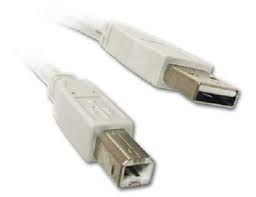
\includegraphics[width=5cm]{figures/5/1174070/teori/1.jpg}
            \centering
            \caption{Membuat file csv}
        \end{figure}

        \item Lalu pada bagian kanan didesktop PC anda, akan muncul popup “Installing device driver software” seperti pada gambar dibawah ini.
        \begin{figure}[H]	
            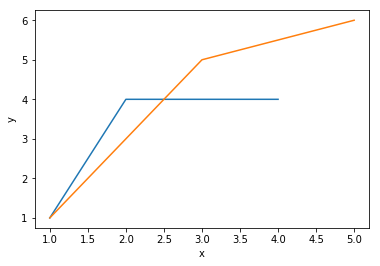
\includegraphics[width=5cm]{figures/5/1174070/teori/2.png}
            \centering
            \caption{Membuat file csv}
        \end{figure}

        \item Tunggu hingga selesai.
        \item Jika sudah selesai anda bisa mengecheck di device manager.
        \begin{figure}[H]	
            \includegraphics[width=5cm]{figures/5/1174070/teori/11.png}
            \centering
            \caption{Membuat file csv}
        \end{figure}
    \end{itemize}

    \item Cara Manual

    \begin{itemize}
        \item Penginstalan secara manual akan dilakukan jika penginstalan secara auto gagal dilakukan.
        \item Buka Device Manager, caranya pada bagian Search Program and Files lalu ketikkan “device manager”, perhatikan gambar dibawah ini. Pada bagian Control Panel akan muncul Device Manager, klik untuk menjalankan.
            \begin{figure}[H]	
                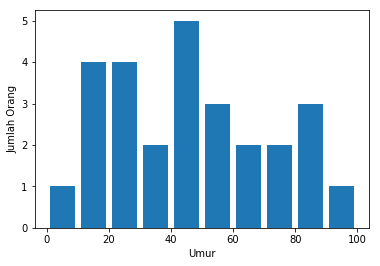
\includegraphics[width=5cm]{figures/5/1174070/teori/4.png}
                \centering
                \caption{Membuat file csv}
            \end{figure}

        \item Cari Unknown device pada bagian Other device, biasanya terdapat tanda seru berwarna kuning, itu disebabkan karena penginstallan tidak berjalan dengan sempurna.
        \begin{figure}[H]	
            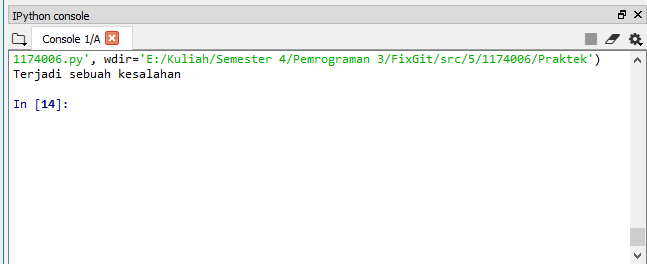
\includegraphics[width=5cm]{figures/5/1174070/teori/5.png}
            \centering
            \caption{Membuat file csv}
        \end{figure}

        \item Klik kanan pada “Unknown device” kemudian pilih Update Driver Software.
        \begin{figure}[H]	
            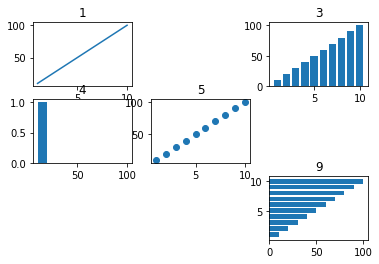
\includegraphics[width=5cm]{figures/5/1174070/teori/6.png}
            \centering
            \caption{Membuat file csv}
        \end{figure}

        \item Pilih Browse my computer for driver software.
        \begin{figure}[H]	
            \includegraphics[width=5cm]{figures/5/1174070/teori/7.png}
            \centering
            \caption{Membuat file csv}
        \end{figure}

        \item Arahkan lokasi folder ke folder ..arduino-1.0.5 drivers. Pastikan check-box lalu centang include subfolders. Klik Next untuk melanjutkan instalasi driver.
        \begin{figure}[H]	
            \includegraphics[width=5cm]{figures/5/1174070/teori/8.png}
            \centering
            \caption{Membuat file csv}
        \end{figure}

        \item Kemudian lanjutkan dengan mengklik Install pada tampilan Windows Security.
        \begin{figure}[H]	
            \includegraphics[width=5cm]{figures/5/1174070/teori/9.png}
            \centering
            \caption{Membuat file csv}
        \end{figure}

        \item Jika instalasi driver berhasil maka akan muncul Windows has successfully updated your driver software.
        \begin{figure}[H]	
            \includegraphics[width=5cm]{figures/5/1174070/teori/10.png}
            \centering
            \caption{Membuat file csv}
        \end{figure}

        \item Perhatikan dan ingat nama COM Arduino Uno, karena nama COM ini yang akan digunakan untuk meng-upload program nantinya.
        \begin{figure}[H]	
            \includegraphics[width=5cm]{figures/5/1174070/teori/11.png}
            \centering
            \caption{Membuat file csv}
        \end{figure}
        \end{itemize}
\end{enumerate}
\subsubsection{Jelaskan bagaimana cara membaca baudrate dan port dari komputer yang sudah terinstall driver}
Untuk baudrate itu bisa dicek melalui arduino IDE, kemudian untuk mengecheck port bisa dilakukan dengan device manager

\subsubsection{Jelaskan sejarah library pyserial}
Modul ini merangkum akses untuk port serial. Ini menyediakan backends untuk Python yang berjalan di Windows, Linux, BSD (mungkin sistem yang mendukung POSIX), Jython dan IronPython (.NET dan Mono). Modul bernama "serial" secara otomatis memilih backend yang sesuai. Antarmuka berbasis kelas yang sama pada semua platform yang didukung.
Akses ke pengaturan port melalui properti Python.
Dukungan untuk berbagai ukuran byte, bit stop, paritas dan kontrol aliran dengan RTS / CTS dan / atau Xon / Xoff.
Bekerja dengan atau tanpa menerima batas waktu.
File seperti API dengan "read" dan "write" ("readline" dll. Juga didukung).
File-file dalam paket ini adalah 100 persen Python murni.
Port diatur untuk transmisi biner. Tidak ada stripping byte NULL, terjemahan CR-LF dll. (Yang berkali-kali diaktifkan untuk POSIX.) Ini membuat modul ini bermanfaat secara universal.
Kompatibel dengan pustaka io (Python 2.6+)

\subsubsection{Jelaskan fungsi-fungsi apa saja yang dipakai dari library pyserial}


Serial – fungsi ini untuk membuka port serial
Write(data) – untuk menulis data lewat port serial
Readline() – untuk membaca string dari port serial
Read(size) – untuk membaca jumlah byte dari port serial
Close() – ini untuk menutup port serial 

\subsubsection{Jelaskan kenapa butuh perulangan dan tidak butuh perulangan dalam membaca serial}


Perualangan dalam bahasa pemrograman berfungsi menyuruh komputer melakukan sesuatu secara berulang-ulang. Terdapat dua jenis perualangan dalam bahasa pemrograman python, yaitu perulangan dengan for dan while.
Perulangan for disebut counted loop (perulangan yang terhitung), sementara perulangan while disebut uncounted loop (perulangan yang tak terhitung). Perbedaannya adalah perulangan for biasanya digunakan untuk mengulangi kode yang sudah diketahui banyak perulangannya. Sementara while untuk perulangan yang memiliki syarat dan tidak tentu berapa banyak perulangannya.
Perulangan diperlukan agar dapat membaca data secara berulang kali sehingga data yang muncul lebih dari satu.  Sedangkan apabila tidak memakai perulangan maka data akan terbaca satu kali saja.

\subsubsection{Jelaskan bagaimana cara membuat fungsi yang mengunakan pyserial}


Berikut merupakan contoh penggunaan fungsi yang menggunakan pyserial
\lstinputlisting[firstline=8, lastline=15]{src/5/1174070/Teori/1174070.py}

\subsubsection{Scan Plagiarisme}
\begin{figure}[H]	
    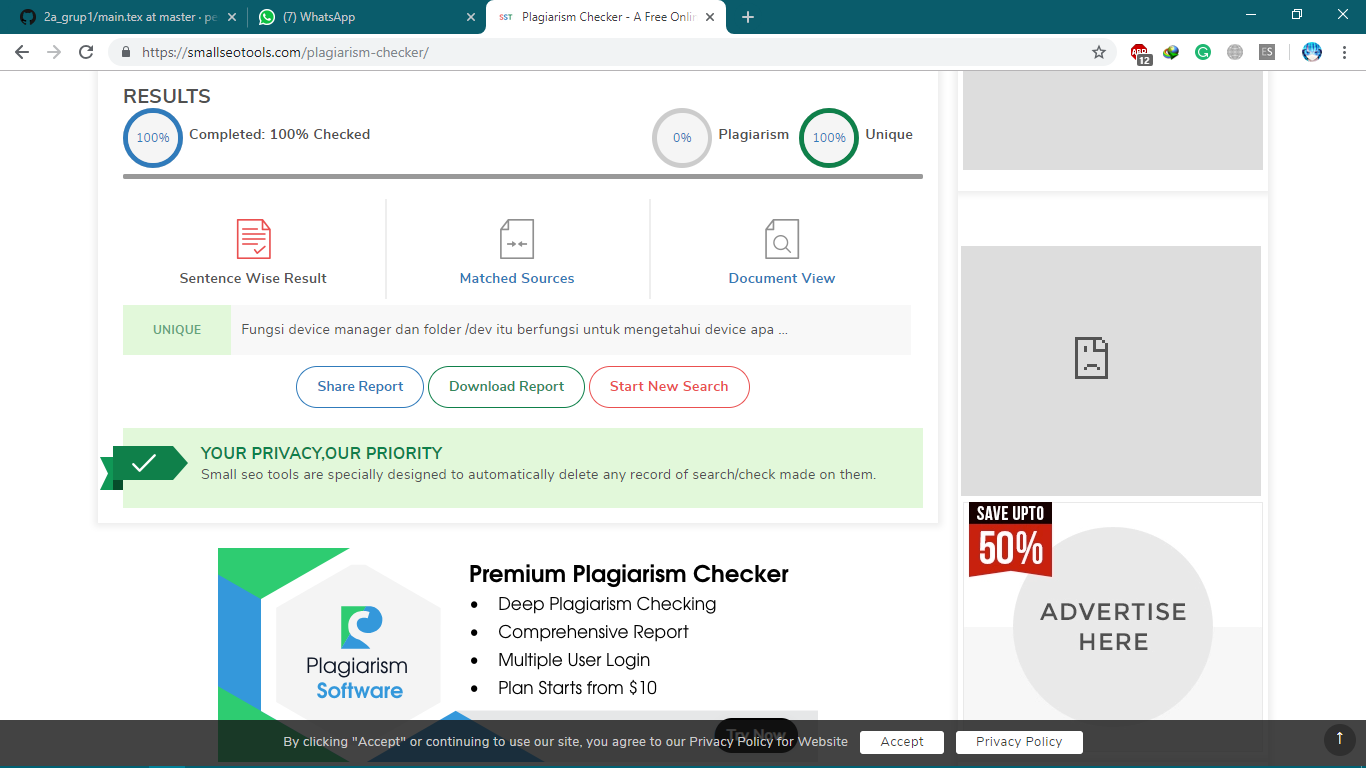
\includegraphics[width=5cm]{figures/5/1174070/Teori/nopla.png}
    \centering
    \caption{Membuat file csv}
\end{figure}

\subsection{Praktek}
\subsubsection{Buatlah fungsi (file terpisah/library dengan nama NPM realtime.py) untuk mendapatkan data langsung dari arduino}
\lstinputlisting[firstline=8, lastline=14]{src/5/1174070/praktek/1174070_realtime.py}

\subsubsection{Buatlah fungsi (file terpisah/library dengan nama NPM save.py) untuk mendapatkan data langsung dari arduino dengan looping}
\lstinputlisting[firstline=8, lastline=15]{src/5/1174070/praktek/1174070_save.py}

\subsubsection{Buatlah fungsi (file terpisah/library dengan nama NPM realtime.py) untuk mendapatkan data dari arduino dan langsung ditulis kedalam file csv}
\lstinputlisting[firstline=16, lastline=29]{src/5/1174070/praktek/1174070_realtime.py}

\subsubsection{Buatlah fungsi (file terpisah/library dengan nama NPM csv.py) untuk membaca file csv hasil arduino dan mengembalikan ke fungsi}
\lstinputlisting[firstline=8, lastline=16]{src/5/1174070/praktek/1174070_csv.py}

\subsubsection{Penanganan Error}
Untuk kali ini saya menemukan Type Error, yaitu error yang menampilkan jika type data na berbeda berusaha disatukan.
\lstinputlisting[firstline=8, lastline=17]{src/5/1174070/praktek/1174070.py}

%%%%%%%%%%%%%%%%%%%%%%%%%%%%%%%%%%%%%%%%%%%%%%%%%%%%%%%%%%%%%%%%%%%%%%%%%%%%%%%%%%%%%%%%%%%%%%%%%%%%%%%%%%%%%%%%%%%%%%%%%

\section{Muhammad Reza Syachrani / 1174084}
\subsection{Pemahaman Teori}
\begin{enumerate}
    \item fungsi device manager di windows adalah membantu dalam mengelola hardware yang terpasang dalam suatu sistem windows. Sedangkan folder /dev pada linux merupakan direktori yang berfungsi untuk menyimpan konfigurasi device atau hardware dari sistem
    \item langkah-langkah instalasi driver Arduino :
    \begin{enumerate}
        \item Hubungkan sistem Arduino Uno ke computer dengan kabel USB type B
        \item lalu akan muncul popup “Installing device driver software” pada bagian kanan dideskop PC.
        \item Namun, sistem operasi windows tidak menyediakan driver untuk Arduino Uno, sehingga proses instalasinya dilakukan secara manual. Dengan cara membuka Device Manager, pada bagian Search Program and Files kita ketikkan device manager lalu klik
        \item Kemudian cari Other device, kemudian klik dan pilih Unkonown device biasanya bertanda seru berwarna kuning, karena penginstalan tidak berjalan sempurna.
        \item Lalu klik kanan pada “Unknown device” dan pilih Update Driver Software
        \item Pilih Browser my computer for driver software
        \item Lalu arahkan lokasi folder ke \ arduino-1.0.5\ driver. Dan pastikan check-box include subfolder dicentang, kemudian klik next.
        \item Dan lanjut mengklik Install pada tampilan Windows Security
        \item Terakhir akan muncul Windows has successfully update your driver software jika instalasi driver berhasil
        \item Dan ingat nama COM Arduino Uno, karena nama COM yang digunakan untuk meng-upload program nantinya.
    \end{enumerate}
    \item Cara membaca baudrate bisa dilihat menggunakan Arduino Ide dengan cara mengklik icon serial monitor , sedangkan port dapat  dilihat pada device manager
    \item pyserial merupakan sebuah serial module/library yang merangkum akses untuk port serial. Ini menyediakan backends untuk Python yang berjalan di Windows, Linux, BSD. Modul bernama "serial" secara otomatis memilih backend yang sesuai. Pyserial pertama kali diluncurkan pada tahun 2002.
    \item Fungsi-fungsi pada library Pyserial :
    \begin{enumerate}
        \item Serial(), berfungsi untuk membuka port serial
        \item write(), Berfungsi untuk mengirimkan data string ke port serial
        \item readline(), Berfungsi untuk membaca sebuah string dari port serial. 
        \item read(size), Berfungsi untuk membaca data dari port serial
        \item close(), Berfungsi untuk menutup port serial
    \end{enumerate}
    \item Perulangan dibutuhkan saat membaca serial, karena agar data yang dibaca tidak hanya satu kali saja tetapi berkali kali, sehingga dengan adanya perulangan tersebut kita dapat membaca datanya berulang kali. Sedangkan perulangan tidak dibutuhkan ketika kita hanya membutuhkan datanya hanya satu. 
    \item cara membuat fungsi menggunakan pyserial:
    \begin{enumerate}
        \item pertama mengimport library serial dengan cara "import serial"
        \item kemudian membuat fungsi dengan mendefinisikan nama fungsi dengan cara def namafungsi():
        \item lalu masukan isi fungsi dengan library pyserial, seperti serial(), read(), dll.
        \item setelah itu panggil namafungsi().
    \end{enumerate}
    \item Scan Plagiarisme
    \begin{figure}[ht!]
    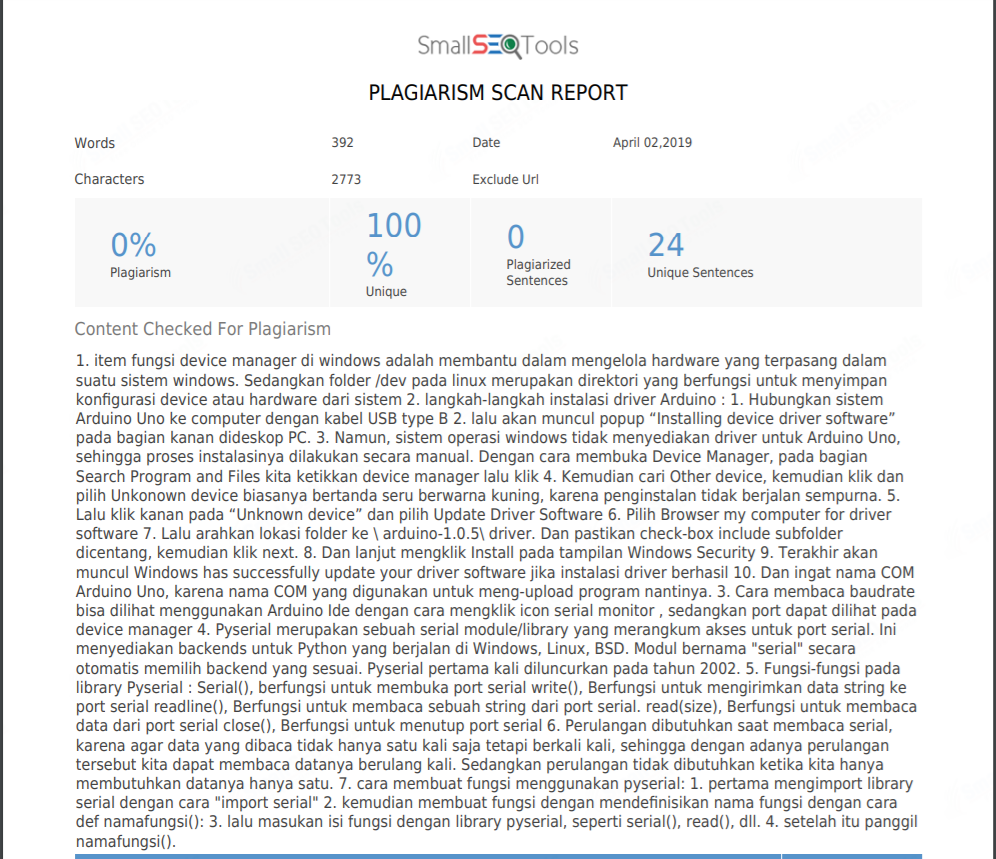
\includegraphics[width=5cm]{figures/5/1174084/Teori/c5_1.png}
    \centering
    \caption{plagiarisme}
    \end{figure}

\end{enumerate}

%%%%%%%%%%%%%%%%%%%%%%%%%%%%%%%%%%%%%%%%%%%%%%%%%%%%%%%%%%%%%%%%%%%%%%%%%%%%%
\section{Ilham Muhammad Ariq}
\subsection{Teori}
\begin{enumerate}
    \item Apa itu fungsi device manager di windows dan folder /dev di linux.
   \par Device Manager dalam komputer Windows, adalah perluasan dari Microsoft Management Console. Device Manager menampilkan seluruh hardware yang bisa di-inisialisasi (dikenali) oleh Windows. Tampilannya sudah ter-organisir (dikelompokkan) sedemikian rupa sehingga akan memudahkan pengelolaan setiap hardware yang ada.Device Manager akan sangat membantu dalam mengelola (manage) semua hardware yang terpasang (dan terdeteksi) dalam suatu sistem Windows. Hardware seperti harddisk, kartu VGA, sound, keyboard, perangkat USB dll. akan sangat mudah untuk dikonfigurasi dari dalam Device Manager ini.
    
    
    \par Folder /dev di linux ialah Directory yang berisi file device, baik device blok maupun device karakter. di dalamnya minimal harus ada file biner MAKEDEV untuk membuat device ini secara manual.

    \item Jelaskan langkah-langkah instalasi driver dari arduino UNO di Windows
  	\par Berikut ini adalah langkah-langkah instalasi driver dari arduino UNO di Windows
	\begin{enumerate}
		\item Pertama pastikan Arduino IDE telah terinstall.		
		\item Hubungkan sistem minimun Arduino Uno ke komputer dengan kabel USB type B (kabel Printer).	
		\begin{figure}[ht]
				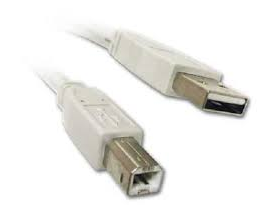
\includegraphics[width=7cm]{figures/5/1174087/Teori/1.png}
				\centering
				\caption{Menghubungkan Port.}
		\end{figure}		
		\item Lalu pada bagian kanan didesktop PC anda, akan muncul popup “Installing device driver software” seperti pada gambar dibawah ini.
		\begin{figure}[ht]
				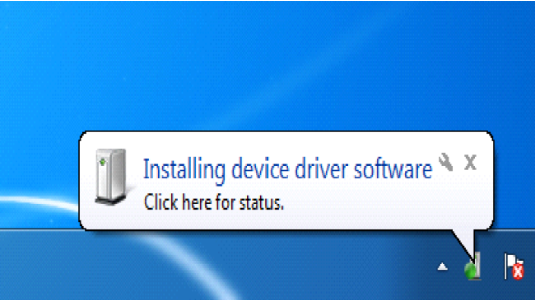
\includegraphics[width=7cm]{figures/5/1174087/Teori/2.png}
				\centering
				\caption{Muncul Pop up.}
		\end{figure}	
		\item Sistem operasi Windows tidak menyediakan driver untuk Arduino Uno seperti yang terlihat pada gambar dibawah ini, lalu proses instalasinya harus dilakukan secara manual.
		\begin{figure}[ht]
				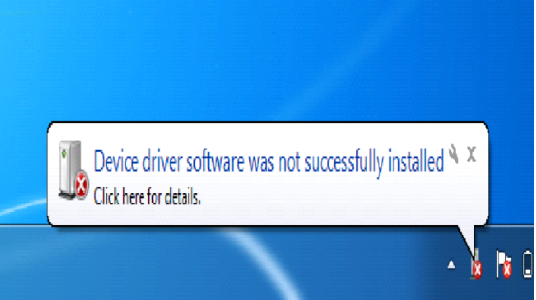
\includegraphics[width=7cm]{figures/5/1174087/Teori/3.png}
				\centering
				\caption{Pop up instalasi Manual.}
		\end{figure}
		\item Buka Device Manager, caranya pada bagian Search Program and Files lalu ketikkan “device manager” (tanpa tanda petik), perhatikan gambar dibawah ini. Pada bagian Control Panel akan muncul Device Manager, klik untuk menjalankan.
		\begin{figure}[ht]
				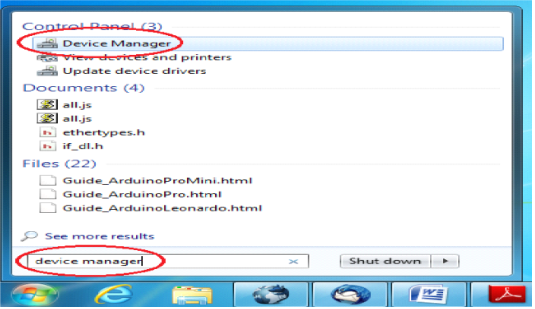
\includegraphics[width=7cm]{figures/5/1174087/Teori/4.png}
				\centering
				\caption{membuka Device Manager.}
		\end{figure}
	\item Cari Unknown device pada bagian Other device, biasanya terdapat tanda seru berwarna kuning, itu disebabkan karena penginstallan tidak berjalan dengan sempurna.
		\begin{figure}[ht]
				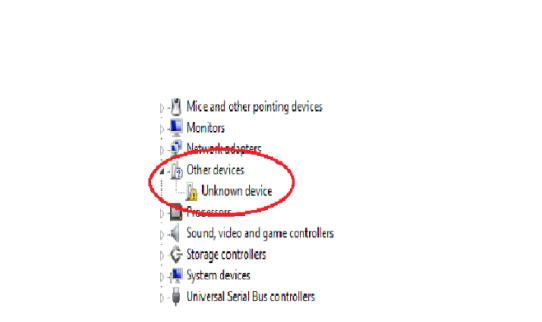
\includegraphics[width=7cm]{figures/5/1174087/Teori/5.png}
				\centering
				\caption{Cari Unknown Device.}
		\end{figure}
		\item Klik kanan pada “Unknown device” kemudian pilih Update Driver Software.
		\begin{figure}[ht]
				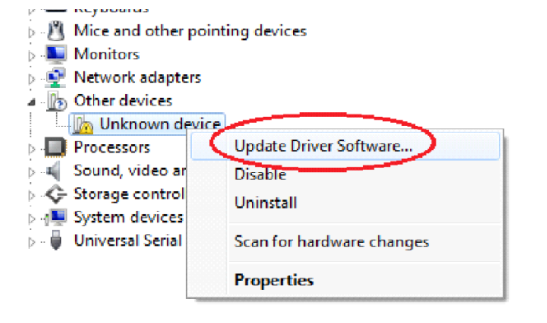
\includegraphics[width=7cm]{figures/5/1174087/Teori/6.png}
				\centering
				\caption{Update Driver Software.}
		\end{figure}
		\item Pilih Browse my computer for driver software.
		\begin{figure}[ht]
				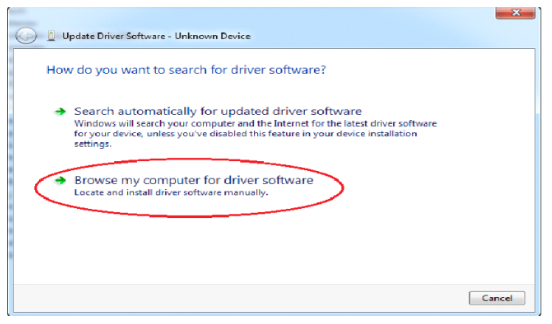
\includegraphics[width=7cm]{figures/5/1174087/Teori/7.png}
				\centering
				\caption{Pilih \textit{Browse my computer for driver software}}
		\end{figure}
		\item Arahkan lokasi folder ke folder \verb|..\arduino-1.0.5\drivers.| Pastikan check-box lalu centang include subfolders. Klik Next untuk melanjutkan instalasi driver.
		\begin{figure}[ht]
				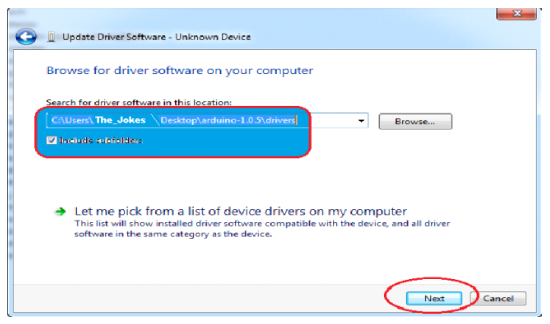
\includegraphics[width=7cm]{figures/5/1174087/Teori/8.png}
				\centering
				\caption{Instalasi Driver}
		\end{figure}
		\item Kemudian lanjutkan dengan mengklik Install pada tampilan Windows Security.
		\begin{figure}[ht]
				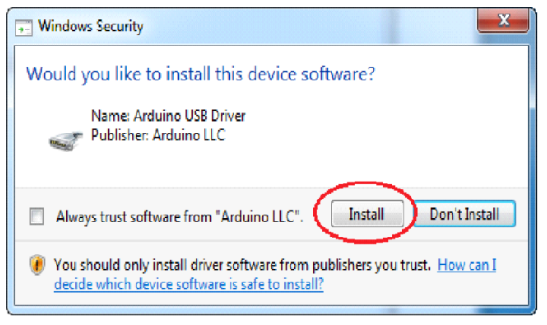
\includegraphics[width=7cm]{figures/5/1174087/Teori/9.png}
				\centering
				\caption{Klik Install}
		\end{figure}
		\item  Jika instalasi driver berhasil maka akan muncul Windows has successfully updated your driver software.
		\begin{figure}[ht]
				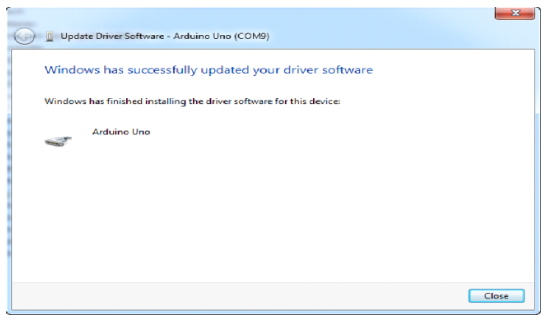
\includegraphics[width=7cm]{figures/5/1174087/Teori/10.png}
				\centering
				\caption{Muncul \textit{Windows has successfully updated your driver software}}
		\end{figure}
		\item Perhatikan dan ingat nama COM Arduino Uno, karena nama COM ini yang akan digunakan untuk meng-upload program nantinya.
			\begin{figure}[ht]
				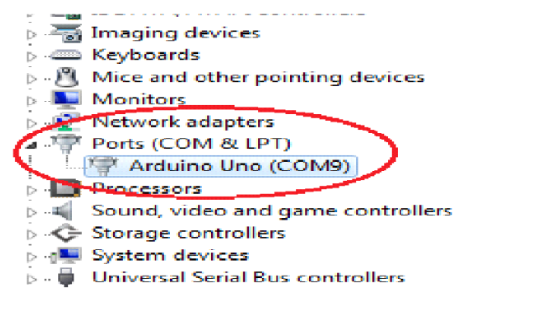
\includegraphics[width=7cm]{figures/5/1174087/Teori/11.png}
				\centering
				\caption{Muncul Nama Arduino}
		\end{figure}
	\end{enumerate}	    
    
    \item Jelaskan bagaimana cara membaca baudrate dan port dari komputer yang sudah
terinstall driver

\par Untuk melihat atau cara membaca baudrate dan port, hanya perlu menginstall Arduino IDE, kemudian membuka menu serial monitor yang berada di tab tools. Selanjutnya akan terlihat baudrate dan port yang sedang digunakan oleh arduino anda.
	
	\item Jelaskan sejarah library pyserial
	
	\par pySerial adalah modul API Python untuk mengakses port serial. pySerial menyediakan API yang seragam di berbagai sistem operasi, termasuk Windows, Linux, dan BSD. PySerial merupakan sebuah library yang digunakan untuk komunikasi ke port serial terutama untuk mikrokontroller. PySerial pertama kali diluncurkan pada tahun 2002 yang makin berkembang dalam setiap versinya hingga tahun 2017 lalu.


	\item Jelaskan fungsi-fungsi apa saja yang dipakai dari library pyserial
	
\par Fungsi-fungsi yang ada pada library PySerial :

\begin{enumerate}
	\item Serial - fungsi ini untuk membuka port serial.
	\item read(size) - fungsi ini untuk membaca jumlah byte dari port serial.
	\item write(data) - fungsi ini menulis data lewat port serial.
	\item readline() - fungsi ini membaca sebuah string dari port serial.
	\item close() - fungsi ini untuk menutup port serial.
\end{enumerate}

	\item Jelaskan kenapa butuh perulangan dan tidak butuh perulangan dalam membaca serial
	
	\par Didalam pembacaan serial pada arduino yang memerlukan membaca data secara berulang-ulang harus dengan perulangan. dan tidak membutuhkan perulangan ketika membaca data hanya dilakukan satu kali saja.
	
	\item Jelaskan bagaimana cara membuat fungsi yang mengunakan pyserial
	\begin{itemize}
	\item import library pyserial dengan cara " import serial"
	\item kemudian membuat fungsi
	\item buat object yang didalamnya ada kelas dan method serial
	\item print object
	\item jalankan kelas
	\end{itemize}	
	
	\item Screenshoot Check Plagiarisme

\begin{figure}[ht]
 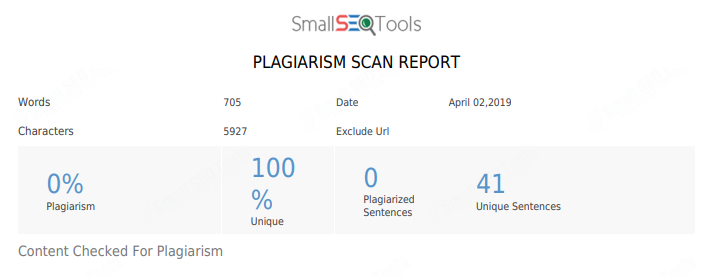
\includegraphics[width=7cm]{figures/5/1174087/Teori/plg.png}
 \centering
 \caption{Screenshoot Check Plagiarisme}
\end{figure}	
	
	\end{enumerate}

%%%%%%%%%%%%%%%%%%%%%%%%%%%%%%%%%%%%%%%%%%%%%%%%%%%%%%%%%%%%%%%%%%%%%%%%%%%%%%%%%%%%%%%%%%%%%%%%